\documentclass[a4paper,12pt]{article}

% --- Pakete ---
\usepackage{tikz}
\usetikzlibrary{positioning}
\usepackage[utf8]{inputenc}   % Umlaute direkt eingeben
\usepackage[T1]{fontenc}
\usepackage[english]{babel}
\usepackage{lmodern}          % Schöne Schrift
\usepackage{geometry}         % Seitenränder anpassen
\usepackage{booktabs}         % Für schönere Tabellen
\usepackage{array}
\usepackage{setspace}         % Zeilenabstand
\usepackage{graphicx}
\usepackage{caption}
\usepackage{url}
\usepackage{todonotes}
\usepackage{float}
\usepackage{pgfplots}
\usepackage{xfp}      % provides \fpeval for calculations
\usepackage{multirow}
\usepackage[
separate-uncertainty = true,
multi-part-units = repeat
]{siunitx}
\usepackage[hidelinks, bookmarks=true]{hyperref}
\pgfplotsset{compat=1.18}

% --- Einstellungen ---
\geometry{a4paper, margin=2.5cm}
\setstretch{1.25}

% --- Dokument ---
\begin{document}
	
	% Titel
	\begin{center}
		{\LARGE \textbf{Praktikum Hochfrequenz-Schaltungstechnik WS25/26}} \\[1em]
		{\large  \textbf{Bericht}} \\[0.5em]
	\end{center}
	
\begin{center}
	\begin{tabular}{|l|p{4cm}|l|p{4cm}|}
		\hline
		\textbf{Name:} &  Sebastian Grigorevski & \textbf{Matrikelnr.:} &  35690104 \\
		\hline
		\textbf{Versuchsnr.:} & 6 & \textbf{Datum:} & \today \\
		\hline
	\end{tabular}
\end{center}
	
	\vspace{1cm}
	\setcounter{section}{6}  % setzt den Section Zähler auf 1
	\setcounter{subsection}{4}  % setzt den Subsection Zähler auf 5
	\setcounter{subsubsection}{0}  % setzt den Subsubsection Zähler auf 0

	\subsubsection{}
The load impedance $Z_L = 136\,\Omega - j34\,\Omega$ at $f = 145\,\mathrm{MHz}$ is matched to a
system impedance of $Z_0 = 50\,\Omega$ using a series transmission line followed by a parallel
transmission line.

First, the load impedance is normalized with respect to $Z_0$ and plotted in the Smith chart:
\[
z_L = \frac{Z_L}{Z_0} = 2.72 - j0.68.
\]

A series transmission line with characteristic impedance $Z_0$ is then added. Varying its length causes the reflection coefficient to rotate along a constant magnitude circle in the Smith chart. The length is chosen such that the transformed impedance intersects the admittance circle corresponding to $20\,\mathrm{mS}$ as can be seen in the figure below on the left. 
At this point, the impedance is converted to the admittance plane. A parallel transmission
line is connected, and its length is adjusted to move the admittance along a constant admittance
circle until the chart center is reached:
\[
z = 1 + j0.
\]
Thus the length of the series cable length is 24 cm and the parallel length is 31 cm to achieve this matching. 

	\begin{figure}[H]
	\begin{center}
		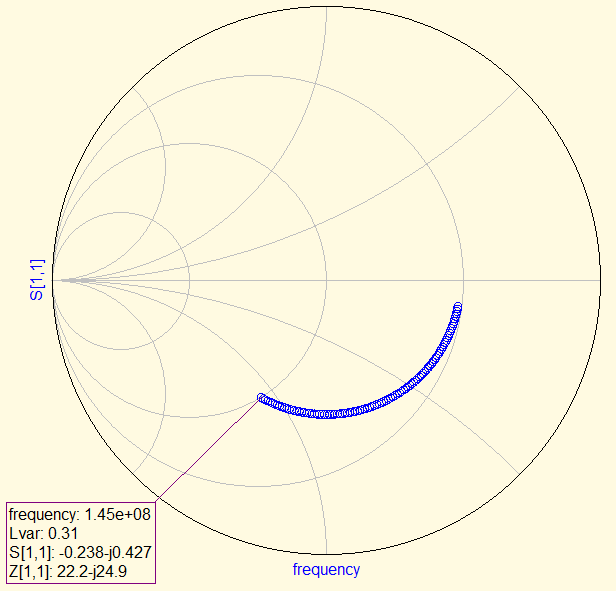
\includegraphics[width=0.44\textwidth]{11.png} 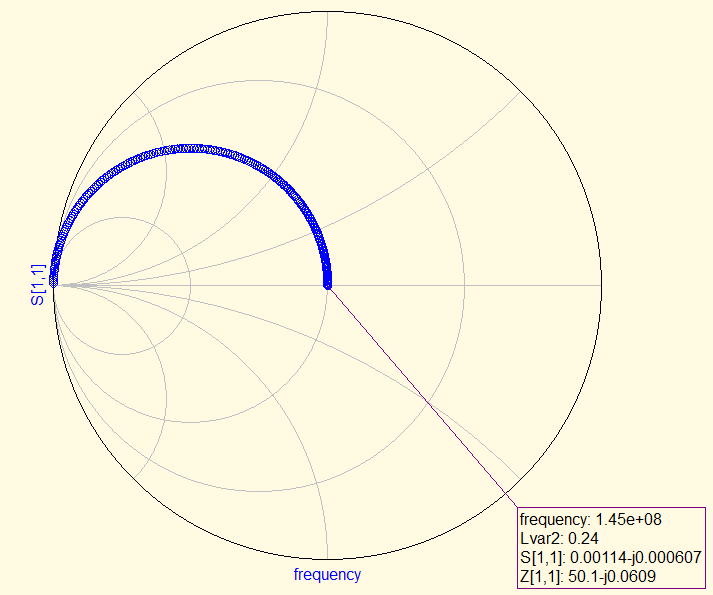
\includegraphics[width=0.5\textwidth]{12.png}
		
	\end{center}
	\caption{Reflection coefficient for increasing series cable length (left) and for increasing parallel cable length (right)} %
	\label{fig:642}
\end{figure}

	
	\subsubsection{}
	For the project \textit{Parallelreihe}, the frequency range is determined in which the difference
	between the input impedance magnitude of the parallel RC network and its series equivalent
	remains below
	\[
	|\Delta Z| < 0.2\,\Omega
	\]
	and simultaneously the phase difference satisfies
	\[
	|\Delta \Phi| < 1^\circ.
	\]
	From the figure \ref{fig:642} the frequency range that satisfies these conditions is determined at $f \in [0.95, 1.1]\,$GHz for a 220 $\Omega$ resistor. The figure shows the differences $\triangle Z = |Z_\mathrm{parallel}-Z_\mathrm{series}|$ and $\triangle \phi = |\phi_\mathrm{parallel}-\phi_\mathrm{series}|$ between the series and parallel circuits.
	\begin{figure}[H]
		\begin{center}
			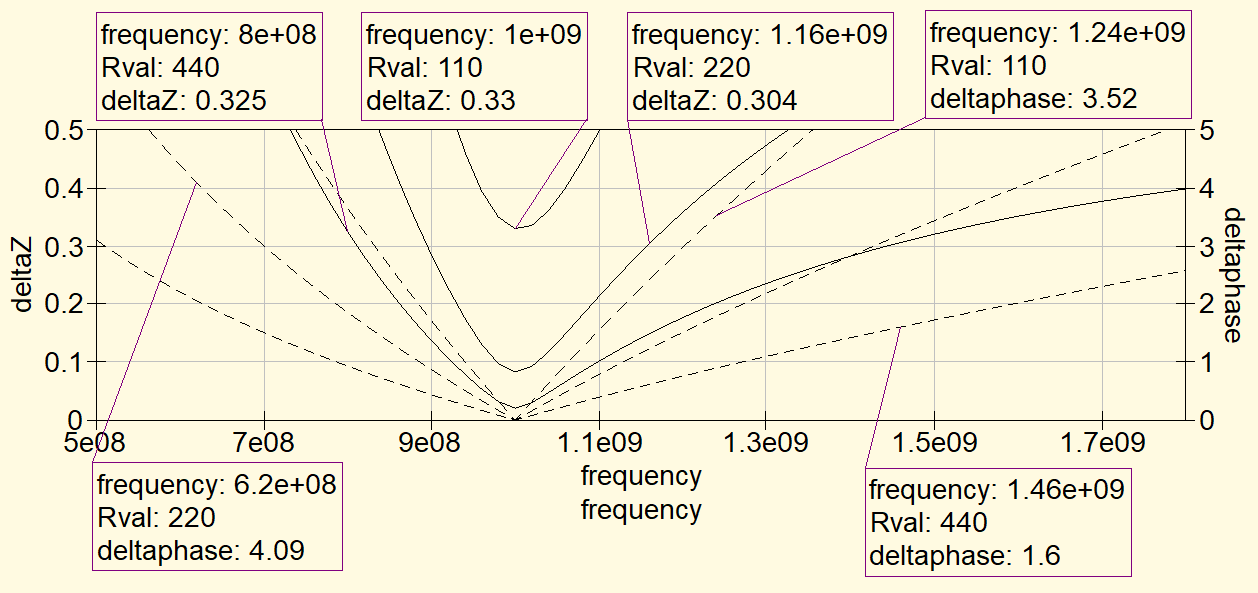
\includegraphics[width=1\textwidth]{642-2.png}
		\end{center}
		\caption{Difference in amplitude in $\Omega$ (solid) and phase in degree (dashed) between a parallel and series circuit as a function of frequency in Hz for different resistances Rval} %
		\label{fig:642}
	\end{figure}
	
	
	When doubling or halving the quality factor by using 110 and 440 $\Omega$ as the parallel resistor and calculating its corresponding series circuits significant changes occur. Looking at the curves for 440 $\Omega$ or double the quality factor the frequency range is larger at $f \in [0.86, 1.24]\,$GHz. On the other hand with 110 $\Omega$ the curve of the amplitude difference lays above the 0.2 $\Omega$ line while the phase curve is also narrower. This behavior supports the validity of the conversion formulas $R_\mathrm{series} = R_\mathrm{parallel}/Q^2$ and $X_\mathrm{series} \approx X_\mathrm{parallel}$ for quality factors $Q > 5$ since the frequency range decreases (diminishes) for smaller quality factors and increases for higher quality factors

	\subsubsection{}	
	For the matching network designed previously, the complex load impedance is removed and the
	reference port is shifted to the right side of the circuit. On the left side of the matching
	network, a resistor of $R=50\,\Omega$ is added to represent the internal resistance of the
	generator. At the design frequency of $f=145\,\mathrm{MHz}$, the simulation yields an input
	impedance of
	\[
	Z_{\mathrm{in}} \approx 136 + j34\,\Omega \, ,
	\]
	corresponding to a magnitude of approximately $140\,\Omega$ with a phase of $14.1^\circ$.
	The resulting input reflection coefficient is
	\[
	|\Gamma| =     X/R \approx 0.25 \, ,
	\]
	indicating a partial mismatch.
	
	This behavior arises because the matching network was designed to transform the complex load
	impedance into $50\,\Omega$ when viewed from the source side. Due to the reciprog network, viewing it from the opposite direction results in the complex conjugate of the
	original load impedance rather than a matched condition.
	
	The type of matching realized by this circuit is therefore a \emph{conjugate impedance match},
	which is valid only in the design direction and at a single frequency \cite{schau_resonanz_komplexe_anpassung_2018}.
	
	\subsubsection{}
	For a lossless transmission line, the input impedance is given by
	\[
	Z_{\mathrm{in}} = Z \frac{Z_L + j Z \tan(\beta l)}{Z + j Z_L \tan(\beta l)} \cite{wiki:Quarter-wave_impedance_transformer}. 
	\] 
	At $l=\lambda/4$, $\tan(\beta l) \rightarrow \infty$, and the expression simplifies to
	\[
	R_{\mathrm{in}} = \frac{Z^2}{R_L} \cite{wiki:Quarter-wave_impedance_transformer}.
	\]
	
	Simulations are performed for different real load resistances
	$R_L = 18\,\Omega, 32\,\Omega, 75\,\Omega, 100\,\Omega, 200\,\Omega$
	and different line impedances
	$Z = 30\,\Omega, 40\,\Omega, 50\,\Omega, \sqrt{5000}\,\Omega, 100\,\Omega$.
	In all cases, the simulated input resistance agrees with the analytical relation within small angle deviations as can be seen in table \ref{tab:lambda4_theory}. At 300 MHz the wavelength is $\lambda = 1$ m, hence $\lambda/4 = 0.25$.
	
	This result shows that a $\lambda/4$ transmission line inverts the load resistance. A low load
	resistance is transformed into a high input resistance and vice versa. By choosing
	\[
	Z = \sqrt{R_{\mathrm{S}} R_L},
	\]
	a perfect impedance match between a source resistance $R_{\mathrm{S}}$ and the load can be
	achieved at the design frequency.
	
	
	\begin{table}[h]
		\centering
		\caption{Simulated and analytical input resistance of a $\lambda/4$ transformer at $f=300\,\mathrm{MHz}$}
		\label{tab:lambda4_theory}
		\begin{tabular}{cccll}
			\hline
			$Z_\text{line}$ [$\Omega$] & $R_L$ [$\Omega$] & $f$ [Hz] & $Z_{11}$ (sim.) [$\Omega/^\circ$] & $R_{\text{in,th}}$ [$\Omega$] \\
			\hline
			30 & 18  & $3\times10^8$ & $50 / -0.0665^\circ$ & 50 \\
			30 & 32  & $3\times10^8$ & $28.1 / 0.00805^\circ$ & 28.1 \\
			30 & 75  & $3\times10^8$ & $12 / 0.131^\circ$ & 12 \\
			30 & 100 & $3\times10^8$ & $9 / 0.189^\circ$ & 9 \\
			30 & 200 & $3\times10^8$ & $4.5 / 0.406^\circ$ & 4.5 \\
			\hline
			40 & 18  & $3\times10^8$ & $88.9 / -0.11^\circ$ & 88.9 \\
			40 & 32  & $3\times10^8$ & $50 / -0.028^\circ$ & 50 \\
			40 & 75  & $3\times10^8$ & $21.3 / 0.0836^\circ$ & 21.3 \\
			40 & 100 & $3\times10^8$ & $16 / 0.131^\circ$ & 16 \\
			40 & 200 & $3\times10^8$ & $8 / 0.299^\circ$ & 8 \\
			\hline
			50 & 18  & $3\times10^8$ & $139 / -0.151^\circ$ & 138.9 \\
			50 & 32  & $3\times10^8$ & $78.1 / -0.0575^\circ$ & 78.1 \\
			50 & 75  & $3\times10^8$ & $33.3 / 0.0519^\circ$ & 33.3 \\
			50 & 100 & $3\times10^8$ & $25 / 0.0935^\circ$ & 25 \\
			50 & 200 & $3\times10^8$ & $12.5 / 0.234^\circ$ & 12.5 \\
			\hline
			70.7 & 18  & $3\times10^8$ & $278 / -0.229^\circ$ & 277.8 \\
			70.7 & 32  & $3\times10^8$ & $156 / -0.109^\circ$ & 156.3 \\
			70.7 & 75  & $3\times10^8$ & $66.7 / 0.00734^\circ$ & 66.7 \\
			70.7 & 50  & $3\times10^8$ & $100 / -0.0441^\circ$ & 100 \\
			70.7 & 100 & $3\times10^8$ & $50 / 0.0441^\circ$ & 50 \\
			70.7 & 200 & $3\times10^8$ & $25 / 0.154^\circ$ & 25 \\
			\hline
			100 & 18  & $3\times10^8$ & $556 / -0.335^\circ$ & 555.6 \\
			100 & 32  & $3\times10^8$ & $312 / -0.175^\circ$ & 312.5 \\
			100 & 75  & $3\times10^8$ & $133 / -0.0363^\circ$ & 133.3 \\
			100 & 50  & $3\times10^8$ & $200 / -0.0935^\circ$ & 200 \\
			100 & 100 & $3\times10^8$ & $100 / 1.4\times10^{-17}{}^\circ$ & 100 \\
			100 & 200 & $3\times10^8$ & $50 / 0.0935^\circ$ & 50 \\
			\hline
		\end{tabular}
	\end{table}
	
	
	
	

	\vfill
	
		
	% --- Bibliography ---
	\bibliographystyle{plain}
	\bibliography{referenzen}
	
	
\end{document}